\section{Strukturorientierte Testverfahren}\label{sec:strukturorientierte-testverfahren}
\begin{tcolorbox}
Bei \textbf{strukturorientierten Testverfahren}, auch \textbf{White-Box-Tests} genannt, wird zur \textbf{Konstruktion der Testfälle} als auch zur \textbf{Bestimmung der Vollständigkeit} der Tests der Quellcode herangezogen.
\end{tcolorbox}

\noindent
Dadurch soll sichergestellt werden, dass jede existierende Codezeile in Tests ausgeführt worden ist.\\
Wird Code in Tests nicht ausgeführt, ist nicht bekannt, ob dieser funktioniert oder nicht - was auch darauf hinweisen könnte, dass der Code nicht erreichbar und damit überflüssig ist, oder ob es sich um einen Defekt handelt.

\subsubsection*{Überdeckungskriterien}
Unter \textbf{vollständiger Überdeckung} des Quellcodes versteht man häufig, dass jede Zeile des Quellcodes einmal ausgeführt wird.\\
Allerdings kann die Vollständigkeit von Tests auch dadurch charakterisiert werden, dass jede \textbf{Verzweigung} mindestens einmal durchlaufen werden muss.\\
Im Folgenden beschränkt sich \textit{Wedemann} auf Kriterien, die zur Definition den \textbf{Kontrollfluss} heranziehen (vgl.~\cite[49 f.]{Wed09c}); für diese existieren auch eine Vielzahl von Werkzeugen\footnote{
\textit{Wedemann} weist ebenda auf \textbf{datenflussorientierte Testverfahren}, die sich auf die vollständige Nutzung von Daten in Tests beziehen. Zum Zeitpunkt der Veröffentlichung von \cite{Wed09c} (2009) gibt er an, dass diese zwar vielversprechend sein, es aber kaum Werkzeuge dafür gäbe.
}.

\subsubsection*{Einsatz}
Strukturorientierte Testverfahren werden i.d.R. im \textbf{Modultest} eingesetzt (s. Abschnitt~\ref{sec:v-modell}), teilweise aber auch im Integrationstests.
Bei System- oder Abnahmetests werden eher \textbf{Black-Box-Tests} genutzt (vgl.~\cite[50]{Wed09c}).

\subsubsection*{Werkzeuge}
Für strukturorientierte Tests ist der Einsatz von Werkzeugen notwendig, da eine händische Kontrolle viel zu aufwändig wäre.
Für die praktische Einsetzbarkeit ist außerdem eine gute Integration in die Entwicklungsumgebung wichtig.

\subsection{Anweisungsüberdeckung}
Das einfachste Kriterium ist die \textbf{Anweisungsüberdeckung} (\textit{statement coverage}).

\begin{tcolorbox}[title=Anweisungsüberdeckung]
    Liegt eine \textbf{Anweisungsüberdeckung} vor, wurde im Test \textit{jede} Anweisung mindestens einmal ausgeführt: \textit{Jeder} Knoten eines \textbf{Kontrollflussgraphen} wurde dann mindestens einmal ausgeführt.
\end{tcolorbox}

\subsubsection*{Beispiel}
Als Beispiel sei der Kontrollflussgraph der Methode \code{countVowels()} gegeben (s. Abbildung~\ref{fig:kontrollflussgraph}).\\
Jeder Knoten wird mit den Testdaten \code{txt="A"} mindestens einmal ausgeführt.

\subsubsection*{Effektivität}
Untersuchungen, die für verschiedene fehlerhafte Methoden die Tests ausschließlich nach Überdeckungskriterien konstruiert haben, haben festgestellt, dass die Tests, die die \textbf{Anweisungsüberdeckung} erfüllen, ca. 15\% der Fehler finden\footnote{
\textit{Wedemann} gibt hierfür - wie für alle Kennzahlen nachfolgender Überdeckungskriterien - leider keine Quelle an, vgl.~\cite[51]{Wed09c}.
}.

\subsubsection*{Werkzeugunterstützung}
Für die meisten imperativen Sprachen gibt es kommerzielle und freie Tools zur Messung der Anweisungsüberdeckung.

\subsubsection*{Einsatzgebiet}
\textit{Wedemann} gibt an, dass die Messung der Anweisungsüberdeckung das verbreiteste Verfahren darstellt, es aber alleine nicht ausreicht, und deshalb im Modultest gemeinsam mit \textbf{funktionsorientierten Testverfahren} (\textit{Grey-Box-Test}) eingesetzt wird (vgl.~\cite[51]{Wed09c}, s. a. Abschnitt~\ref{sec:klassentest-objektorientierter-systeme}).

\subsection{Zweigüberdeckung}

Eine \textbf{Zweigüberdeckung} (\textit{branch coverage}) wird erreicht, wenn im Test jede \textit{Verzweigung} einmal ausgeführt worden ist.

\begin{tcolorbox}[title=Zweigüberdeckung]
Eine \textbf{Zweigüberdeckung} liegt vor, wenn \textit{jede} Kante des Kontrollflussgraphen mindestens einmal ausgeführt worden ist.\\
    Liegt eine Zweigüberdeckung vor, ist gleichzeitig auch die \textbf{Anweisungsüberdeckung} erfüllt.
\end{tcolorbox}

\subsubsection*{Beispiel}
Als Beispiel sei der Kontrollflussgraph der Methode \code{countVowels()} gegeben (s. Abbildung~\ref{fig:kontrollflussgraph}).\\
Jeder Knoten wird mit den Testdaten \code{txt="AB"} mindestens einmal ausgeführt - jeder Knoten des Kontrollflussgraphen wird von mindestens einer Kante erreicht.

\subsubsection*{Effektivität}
Untersuchungen haben ergeben, dass Tests, die so konstruiert werden, dass sie die \textbf{Zweigüberdeckung} erfüllen, ca. 30\% der Fehler finden.

\subsubsection*{Werkzeugunterstützung}
Weniger Tools zur Messung der Zweigüberdeckung als Anweisungsüberdeckung im Jahr der Veröffentlichung von \cite{Wed09c} (2009). \textit{Wedemann} gibt Hinweise auf kommerziell verfügbare Werkzeuge, ohne die Werkzeuge näher zu benennen.

\subsection{Pfadüberdeckung}
Die Zweigüberdeckung bietet schon eine ziemlich vollständige Überdeckung, berücksichtigt aber Schleifen nicht genügend.
Das Verhalten des Testgegenstandes beim abweisenden Fall oder bei mehreren Durchläufen der Schleife führen zu der Forderung der Verallgemeinerung der Möglichkeiten: Im Test sollen alle \textit{Pfade}, die durch den Kontrolflussgraphen laufen, vorkommen.
In diesem Fall spricht man von \textbf{Pfadüberdeckung} (\textit{path coverage} bzw. \textit{loop coverage}).
Da es bei Schleifen häufig unendlich viele Pfade gibt (\cite[52]{Wed09c}), wird anstatt der Pfadüberdeckung die \textbf{Boundary-Interior-Überdeckung} gewählt.

\begin{tcolorbox}[title=Boundary-Interior-Coverage]
    Die \textbf{Boundary-Interior-Coverage} ist eine Form der \textbf{Pfadüberdeckung}, bei der bei Schleifen der abweisende Fall (\textit{boundary}) und mindestens zwei Durchläufe (\textit{interior}) genügen.\\
    Wird eine Boundary-Interior-Überdeckung erreicht, ist automatisch auch die \textbf{Zweigüberdeckung} erreicht.
\end{tcolorbox}

\noindent
Boundary-Interior ist allerdings nicht immer erreichbar, da manchmal der \textbf{abweisende Fall} \textit{nicht} provoziert werden kann.\\
\textit{Wedemann} weist darauf hin, dass Boundary-Interior von verschiedenen Autoren und Standards unterschiedlich definiert wird; so wird häufig gefordert, dass die Schleife \textit{genau einmal} durchlaufen werden soll, was aber nicht immer realisiert werden kann (vgl.~\cite[52]{Wed09c}).

\subsubsection*{Beispiel}
Als Beispiel sei der Kontrollflussgraph der Methode \code{countVowels()} gegeben (s. Abbildung~\ref{fig:kontrollflussgraph}).\\
Eine Boundary-Interior-Überdeckung wird mit $5$ Testfällen erreicht:

\begin{itemize}
    \item \textbf{Boundary}: \code{txt = ""} (Schleife wird nicht betreten)
    \item \textbf{Interior} (Schleife wird zweimal betreten, alle möglichen Pfade werden durchlaufen):
    \begin{itemize}
        \item \code{txt="AA"}
        \item \code{txt="AB"}
        \item \code{txt="BA"}
        \item \code{txt="BB"}
    \end{itemize}
\end{itemize}

\subsubsection*{Effektivität}
Untersuchungen haben ergeben, dass die Tests, die so konstruiert werden, dass sie die Boundary-Interior-Überdeckung erfüllen, ca. 60\% der Fehler finden.

\subsubsection*{Werkzeugunterstützung}
Für kommerziell wichtige Sprachen weist \textit{Wedemann} auf kommerziell verfügbare Werkzeuge hin, ohne die Werkzeuge näher zu benennen.

\subsection{Bedingungsüberdeckung}
Die bisherigen Testfälle lassen die im Beispiel der Methode \code{countVowels()} vorhandenen Bedingungen im \code{if}-Statement außer Acht - die bisherigen Testfälle haben allesamt nur $A$ bzw. $B$ berücksichtigt.\\
Die \textbf{Bedingungsüberdeckung} fordert, dass im Test \textit{jede} Bedingung mindestens einmal \textit{wahr} und einmal \textit{falsch} sein muss.\\
Die wichtigste Variante der \textbf{Bedingungsüberdeckung} ist die \textbf{einfache Mehrfachbedingungsüberdeckung} (\textit{modified condition decision coverage}):

\begin{tcolorbox}[title=Einfache Mehrfachbedingungsüberdeckung]
Die \textbf{einfache Mehrfachbedingungsüberdeckung} wird erreicht, wenn \textit{jede} atomare Bedingung, also jeder \textit{direkte Vergleich}, und \textit{alle zusammengesetzten Bedingungen} einmal den Wahrheitswert \textit{wahr} und einmal den Wahrheitswert \textit{falsch} annehmen\footnote{
    \textit{Maxterm}: Für genau eine Variablenbelegung falsch (Disjunktion: $A \lor B \lor C$); bzw. \textit{Minterm}: für genau eine Variablenbelegung wahr (Konjunktion: $A \land B \land C$)(vgl.~\cite[92]{Hof22})
}.\\
    Dadurch wird gleichzeitig eine \textbf{Zweigüberdeckung} erreicht
\end{tcolorbox}

\subsubsection*{Beispiel}
Als Beispiel sei der Kontrollflussgraph der Methode \code{countVowels()} gegeben (s. Abbildung~\ref{fig:kontrollflussgraph}).\\
Eine einfache Mehrfachbedingungsüberdeckung wird mit den Testdaten \code{txt="AEIOUX"} erreicht: Die Vokale in dem String sorgen dafür, dass \textit{jede atomare Bedingung} einmal wahr wird, durch das \code{X} wird einmal der \textit{gesamte Ausdruck} falsch (\code{if (txt.charAt(i) == 'A' || txt.charAt(i) == ...)}).

\subsubsection*{Effektivität}
Untersuchungen haben ergeben, dass die Tests, die so konstruiert werden, dass sie die einfache Mehrfachbedingungsüberdeckung  erfüllen, ca. 60\% der Fehler finden.

\subsubsection*{Werkzeugunterstützung}
\textit{Wedemann} weist auf eine bessere Werkzeugunterstützung als bei der Boundary-Interior-Überdeckung hin (vgl.~\cite[53]{Wed09c}).

\subsection{Vergleich der Überdeckungen}

Die verschiedenen Überdeckungskriterien lassen sich auch hierarchisch darstellen (s. Abbildung~\ref{fig:coverage-criteria-hierarchy}).

\begin{figure}
    \centering
    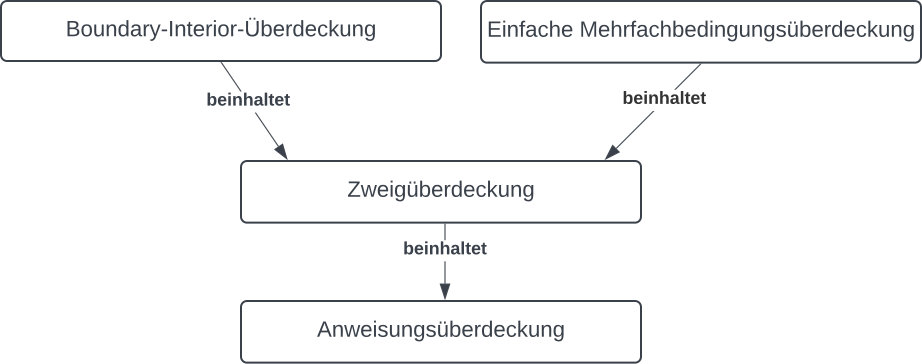
\includegraphics[scale=0.4]{part four/Testende Verfahren/img/coverage-criteria-hierarchy}
    \caption{Hierarchie der verschiedenen Überdeckungskriterien. (Quelle: in Anlehnung an \cite[Abb. 5.2, 53]{Wed09c})}
    \label{fig:coverage-criteria-hierarchy}
\end{figure}

 \noindent
Eine \tectbf{vollständige Überdeckung} zu erreichen ist schwierig.
Bereits eine Anweisungsüberdeckung ist bei \textit{nicht trivialer} Software mit hohem Aufwand verbunden: Forderungen nach höheren Überdeckungen ziehen entsprechend höheren Aufwand nach sich.\\
Man sollte also entscheiden, ob eine vollständige Überdeckung notwendig ist, oder ob eine \textbf{partielle Überdeckung} (z.B. $80$ - $90$\%) ausreichend sein könnte\footnote{
``da [erfahrungsgemäß] die letzte 10-20\% am schwierigsten zu erreichen sind`` (\cite[54]{Wed09c}).
}.\\
Eine vollständige Überdeckung kann auch nur für \textbf{kritische Codeteile} gefordert werden.\\

\noindent
Trotz des hohen Aufwandes ist es gerade bei Software, von der Menschenleben abhängen, notwendig, die Überdeckungskriterien in der Praxis als Werkzeug zu nutzen: Wird im Test die Boundary-Interior-Überdeckung und die einfache Mehrfachbedingungsüberdeckung gleichzeitig erfüllt, sind mit sehr hoher Wahrscheinlichkeit die meisten durch Codierfehler verursachten Defekte entdeckt.\\

\noindent
Coverage-Werkzeuge sind aber in jedem Fall wertvolle Hilfen für Entwickler im \textbf{Modultest}, um die Vollständigkeit der Testfälle zu prüfen.